\documentclass[tikz,border=15pt]{standalone}
\usetikzlibrary{arrows.meta}
\begin{document}
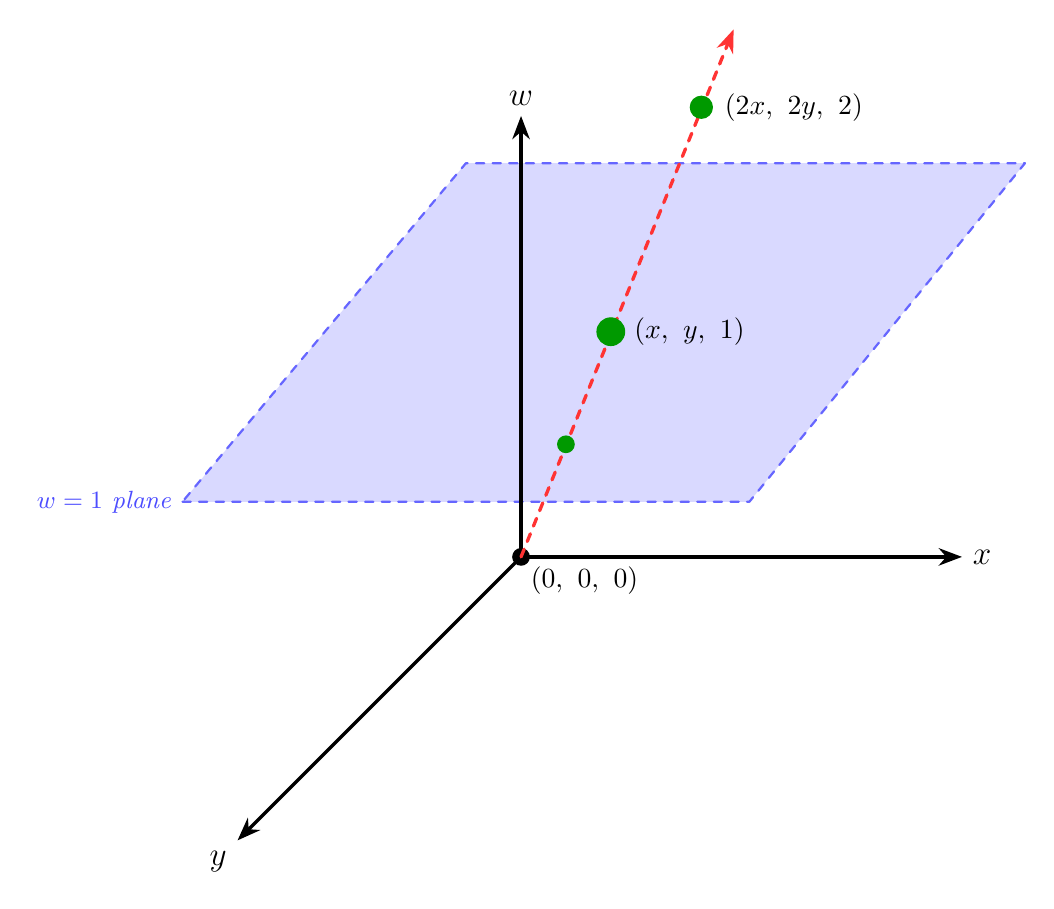
\begin{tikzpicture}[>=Stealth, line cap=round, line join=round, scale=1.0]

    % ── Coordinate mapping from SVG (scale down by ~28) ──────────────────────
    % SVG viewBox: -200 to 200, so we map to roughly -7 to 7 in TikZ
    % SVG x→right, SVG y→down, TikZ y→up so we negate y

    % Axes in SVG:
    %   X: (0,0)→(150,0)       => TikZ: (0,0)→(5.5,0)
    %   Y: (0,0)→(-100,100)    => TikZ: (0,0)→(-3.6,-3.6)
    %   W: (0,0)→(0,-150)      => TikZ: (0,0)→(0,5.5)

    % Plane polygon SVG: -120,-20  80,-20  180,-140  -20,-140
    % TikZ (div 28, negate y):  -4.3,0.7  2.9,0.7  6.4,5.0  -0.7,5.0

    % Ray SVG: (0,0)→(75,-187.5)  => TikZ: (0,0)→(2.7,6.7)
    % P1 SVG:  (32,-80)           => TikZ: (1.14,2.86)
    % P2 SVG:  (64,-160)          => TikZ: (2.29,5.71)
    % P0 SVG:  (16,-40)           => TikZ: (0.57,1.43)

    % ── W=1 Plane (drawn first, behind axes) ─────────────────────────────────
    \filldraw[fill=blue!15, draw=blue!60, thick, dashed]
        (-4.3, 0.7) -- (2.9, 0.7) -- (6.4, 5.0) -- (-0.7, 5.0) -- cycle;

    % Plane label
    \node[font=\small\itshape, blue!70, anchor=east] at (-4.3, 0.7)
        {$w = 1\ \mathit{plane}$};

    % ── Axes ──────────────────────────────────────────────────────────────────
    % X axis
    \draw[->, very thick] (0,0) -- (5.6, 0)
        node[right, font=\large\itshape] {$x$};

    % Y axis (down-left in perspective)
    \draw[->, very thick] (0,0) -- (-3.6, -3.6)
        node[below left, font=\large\itshape] {$y$};

    % W axis (up)
    \draw[->, very thick] (0,0) -- (0, 5.6)
        node[above, font=\large\itshape] {$w$};

    % ── Origin ────────────────────────────────────────────────────────────────
    \filldraw[black] (0,0) circle (3pt);
    \node[below right, font=\normalsize\itshape] at (0,0) {$(0,\ 0,\ 0)$};

    % ── Ray from origin (dashed red) with arrow ───────────────────────────────
    \draw[->, red!80, very thick, dashed] (0,0) -- (2.7, 6.7);

    % ── Points on ray ─────────────────────────────────────────────────────────
    % w=0.5 point (small, no label)
    \filldraw[green!60!black] (0.57, 1.43) circle (3pt);

    % w=1 point — on the plane
    \filldraw[green!60!black] (1.14, 2.86) circle (5pt);
    \node[right=5pt, font=\normalsize\itshape] at (1.14, 2.86)
        {$(x,\ y,\ 1)$};

    % w=2 point
    \filldraw[green!60!black] (2.29, 5.71) circle (4pt);
    \node[right=5pt, font=\normalsize\itshape] at (2.29, 5.71)
        {$(2x,\ 2y,\ 2)$};

\end{tikzpicture}
\end{document}